%!TEX root = ../Systementwurf.tex

\chapter{Einleitung}

\NewsGenie ist der persönliche Nachrichtensprecher. Immer auf dem neuesten
Stand und begierig darauf, die Fragen seiner Nutzer zu beantworten.
"`Was gibt es Neues in Russland?"', "`Wie hat Eintracht
Braunschweig gespielt?"', "`Wie alt ist Angela Merkel?"' - \NewsGenie
versteht seinen Benutzer ohne Tastatur, Suchmaske oder Bildschirm sondern in
völlig normaler Sprache.

Als Thin-Client-Server-Anwendung wird \NewsGenie so realisiert, dass der
Nutzer mittels eines kleinen und günstigen Clients auf das System
zugreifen und seine Anfragen stellen kann. Dabei hat er die Möglichkeit nach
Nachrichten aus einem Bereich, wie \glqq Technologie\grqq\, einem bestimmten aktuellen Thema, wie der Ukraine, sowie nach Fakten,
z.B. dem Alter einer Person des öffentlichen Lebens, zu suchen.

Um dies zu realisieren, wird dem Server eine maßgebliche Rolle zuteil. Dieser verarbeitet die Anfragen der verschiedenen Clients, 
erfasst parallel die einzelnen Nachrichtenartikel von den in der Datenbank
hinterlegten Newsseiten und stellt den Nutzern ein Webinterface zur Verfügung.

Der Server basiert auf einer 3-Schichten-Architektur aus
Benutzerschnittstelle, System- und Persistenzschicht und wird in Java
entwickelt.
Die Benutzerschnittstelle besteht auf der Serverseite aus dem Webinterface, das mit Hilfe des Play-Frameworks\footnote{Mit dem quelloffenen Play-Framework kann man einfach ressourcenschonende Web-Applikationen in Java und Scala entwickeln. \url{http://www.playframework.com/}} realisiert wird.
Die Systemschicht stellt die Kernfunktionalität des Servers bereit, das Annehmen von Anfragen, deren Verarbeitung mit Hilfe von "`Natural Language Processing"'\footnote{Stanford CorNLP, eine Sammlung von Sprachanalysetools. Verwendet werden der Part-of-Speech tagger (POS) und der Named Entity Recognizer (NER), \url{http://nlp.stanford.edu/software/corenlp.shtml}} und außerdem den Crawler, welcher regelmäßig die hinterlegten Newsseiten nach neuen Artikeln durchsucht und in der Persistenzschicht, einer Datenbank realisiert mit einem Virtuoso\footnote{OpenLink Virtuoso ist ein quelloffenes Datenbanksystem, das die Funktionalität vieler verschiedener Datenbankparadigmen kombiniert. Wird hier als Triple-Store verwendet. \url{http://virtuoso.openlinksw.com/dataspace/doc/dav/wiki/Main/}} Triple-Store, speichert. 
Die Datenbank ist außerdem mit einem Lucene-Index versehen.

%
%Die Benutzerschnittstelle besteht auf der Serverseite aus dem Webinterface.
%In diesem kann sich der Benutzer registrieren und nach einem Login Textanfragen stellen
%und seine Nachrichtenquellen verwalten. 
%Weiterhin besteht die Möglichkeit, sein Passwort zu ändern oder wiederherzustellen und 
%seinen Account zu löschen. Administratoren können außerdem in die Sicht von anderen
%Benutzern wechseln und diese löschen. Das Webinterface wird mit Hilfe des Play-Frameworks realisiert.
%
%Die Systemschicht stellt die Kernfunkionalitäten des Servers bereit. Der
%Management-Handler nimmt alle Anfragen von Clients und aus dem Webinterface entgegen 
%und koordinert die weiteren Schritte. Handelt es sich dabei ausschließlich um eine Anfrage nach Daten,
%wie zum Beispiel bei einem Login-Versuch, wo geprüft werden muss, ob ein Nutzername registriert ist, 
%werden diese Informationen aus der Datenbank gesucht und die Anfrage so beantwortet. Handelt es sich 
%jedoch um eine Anfrage nach Neuigkeiten, besteht diese aus natürlicher Sprache und muss zunächst interpretiert werden.
% Hierzu wird die eingegangene Anfrage
% durch "`Natural Language Processing"' analysiert und durch
%unser eigenes Analysetool geschickt, welches die enthaltenen Wörter in einen Kontext setzt.
%Anschließend werden die am Besten zur Anfrage passenden Artikel aus der Datenbank gesucht und das
% Ergebnis wieder in einen natürlichen Satz umgewandelt.
%Außerdem beinhaltet die Systemschicht den Crawler, welcher die in der Datenbank
%hinterlegten Newsseiten regelmäßig nach neuen Artikeln durchsucht.
%
%Die Persistenzschicht beinhaltet einen Virtuoso-Triplestore, der als Datenbank dient, 
%sowie einen Lucene-Index zur effizienten Volltextsuche. 
%In Virtuoso werden die Daten der Benutzer sowie Feeds und deren beinhaltete Artikel gespeichert.

Alle Schichten kommunizieren mit Hilfe des Akka-Frameworks\footnote{Akka ist ein Framework zur Entwicklung fehlertoleranter, verteilter Java- und Scala Anwendungen, basierend auf dem Aktoren-Modell. \url{http://akka.io/}}, welches einen sicheren,
asynchronen Datenaustausch ermöglicht.

Aus der genannten Aufteilung resultieren die in Abb. \ref{komponenten}
dargestellten Komponenten.

In den nachfolgenden Abschnitten wird die Implementierung \NewsGenie vorgestellt. Zunächst die Komponentenaufteilung, gefolgt von Implementierungsdetails wie den einzelnen Funktionen und dem Datenmodell.

\begin{figure}[h]
\centering
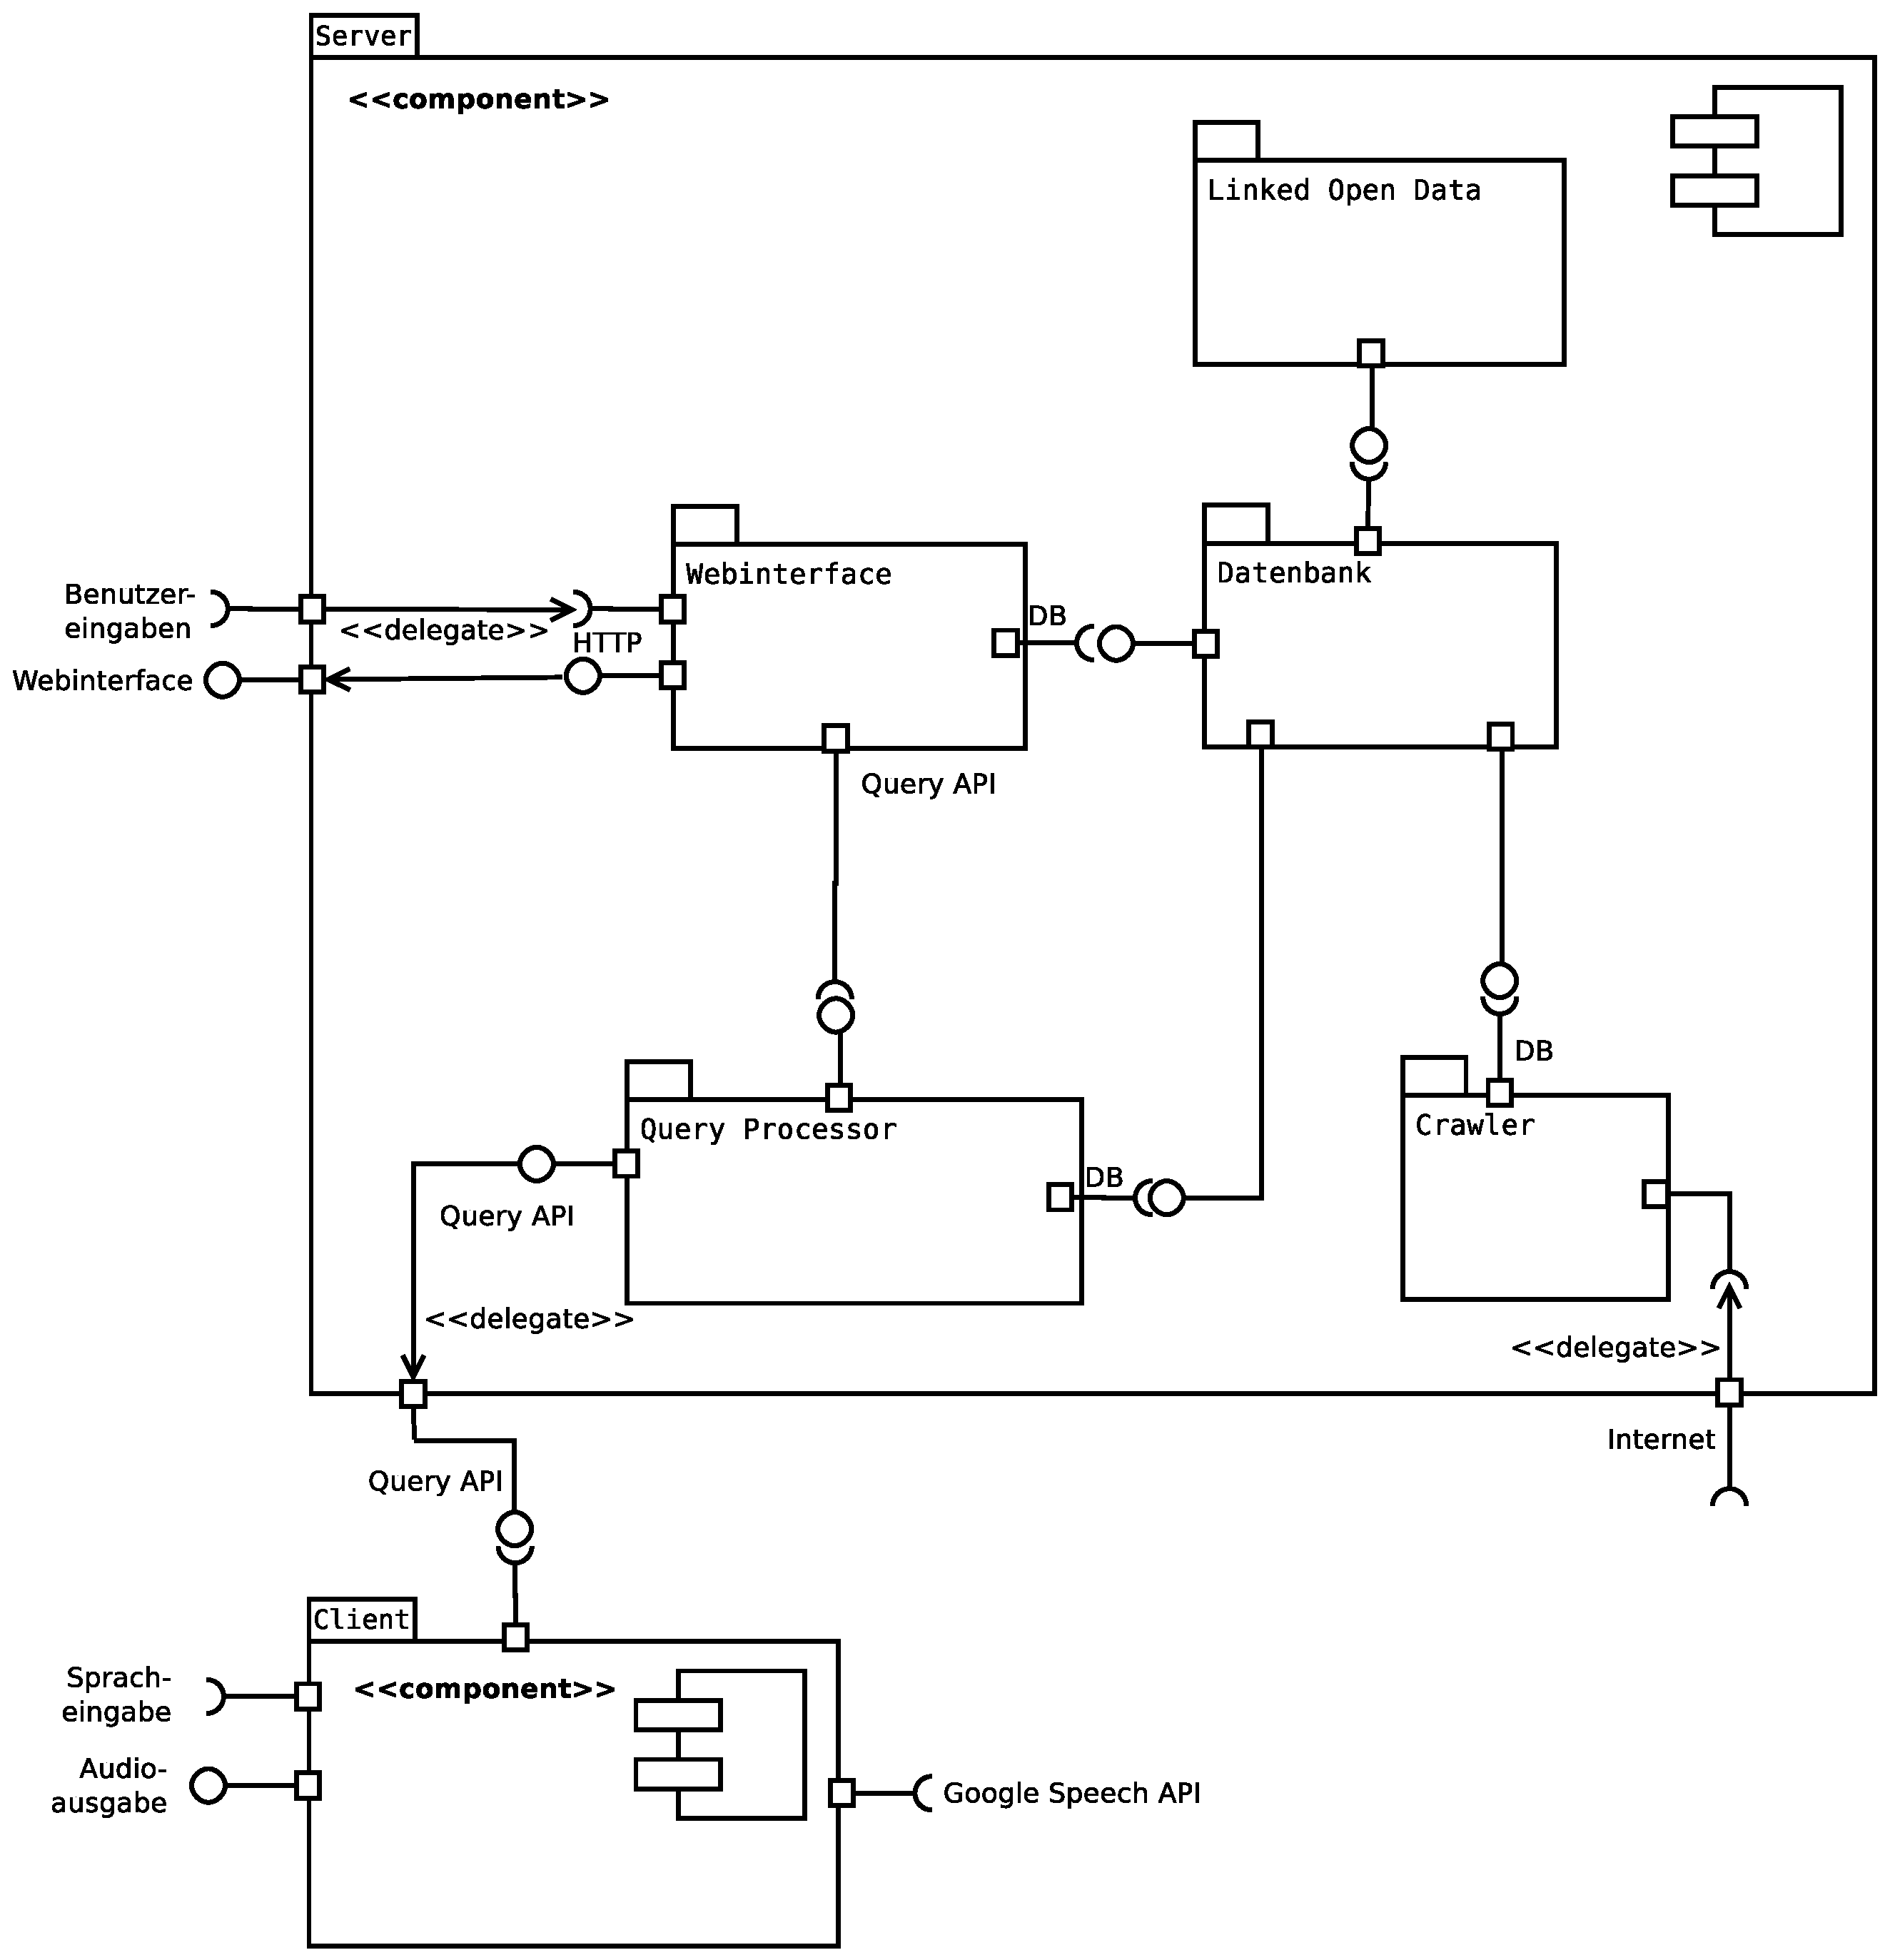
\includegraphics[width=1\textwidth]{Systementwurf/05_implementierungsentwurf/komponenten}
\caption{Komponentendiagramm, \textit{Komponentenaufteilung von \NewsGenie}
\label{komponenten}}
\end{figure}

\FloatBarrier
\section{Projektdetails}

Um wichtige Aspekte von \NewsGenie genauer zu erläutern, werden in diesem
Kapitel verschiedene Funktionen der Anwendung aufgeführt und beschrieben. In den folgenden
Unterkapiteln werden das Registrieren, die Anmeldung am Webinterface, das Hinzufügen von Feeds
 und die Interaktion zwischen Benutzer und Client genauer erklärt.

\subsection{Registrieren und Anmelden}

Die folgenden Aktivitätsdiagramme~\ref{1.2}~und~\ref{1.3} beschreiben den Workflow bei der Registrierung
 und Anmeldung eines Nutzers. Will
sich ein Nutzer registrieren um \NewsGenie zu nutzen, so muss er im Webinterface
den entsprechenden Registrierungs-Button anklicken. Dadurch wird ihm vom System
die Seite angezeigt, auf der er seinen gewüschten Benutzernamen und sein selbst
gewähltes Passwort sowie seine E-Mail-Adresse in Textfelder eintragen kann.
Nachdem der Nutzer seine Eingaben bestätigt hat, legt das System
seine Daten in der Datenbank ab, sofern sie nicht schon vergeben waren.
 Nun kann der Nutzer sich am Client und im
Webinterface anmelden. Über den Client kann er anschließend Anfragen stellen
oder über das Webinterface seine Einstellungen verwalten bzw. eine Textanfrage
stellen.

\begin{figure}[h]
\centering
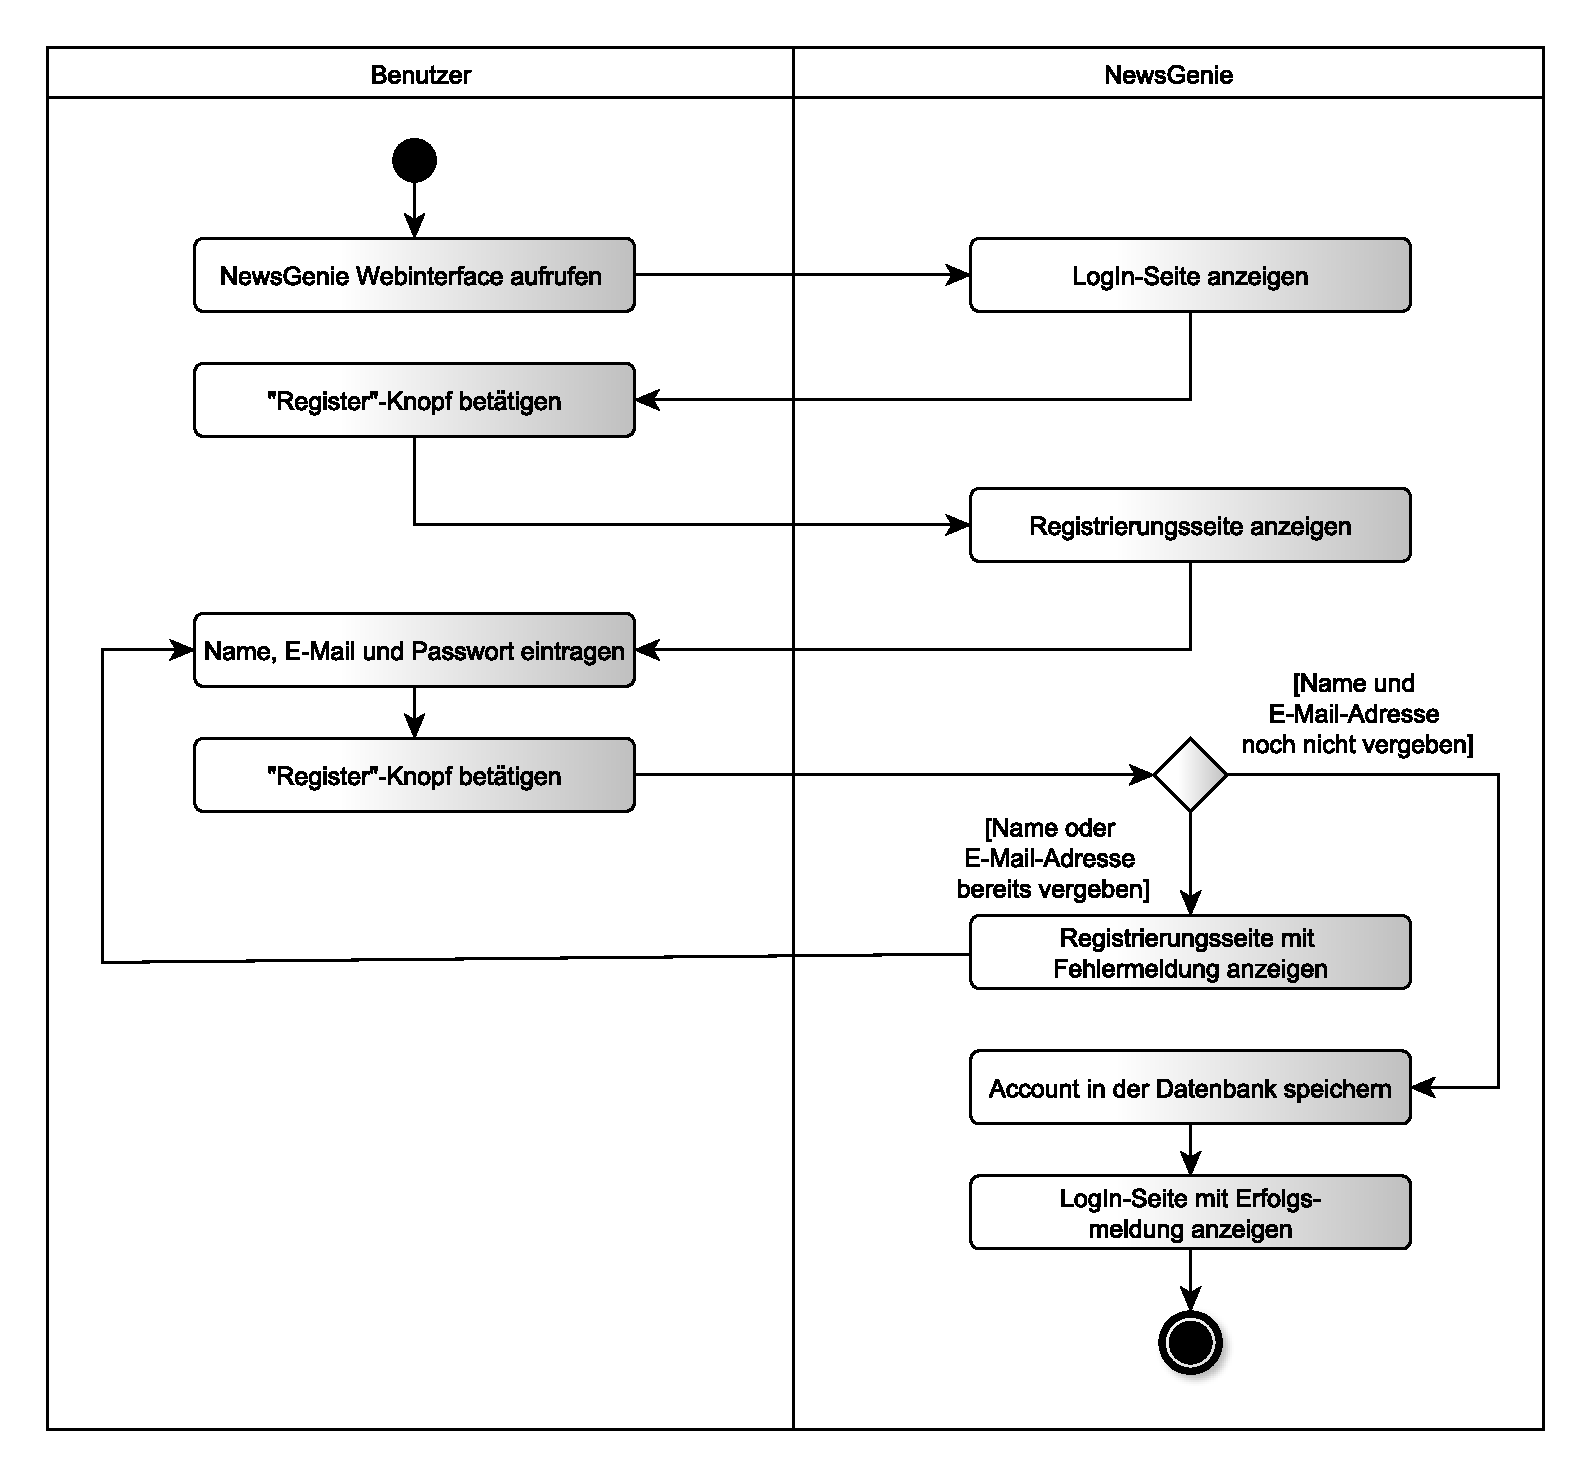
\includegraphics[width=1\textwidth]{Systementwurf/01_einleitung/register.eps}
\caption{Aktivitätsdiagramm, \textit{Registrierung bei \NewsGenie}
\label{1.2}}
\end{figure}

\begin{figure}[h]
\centering
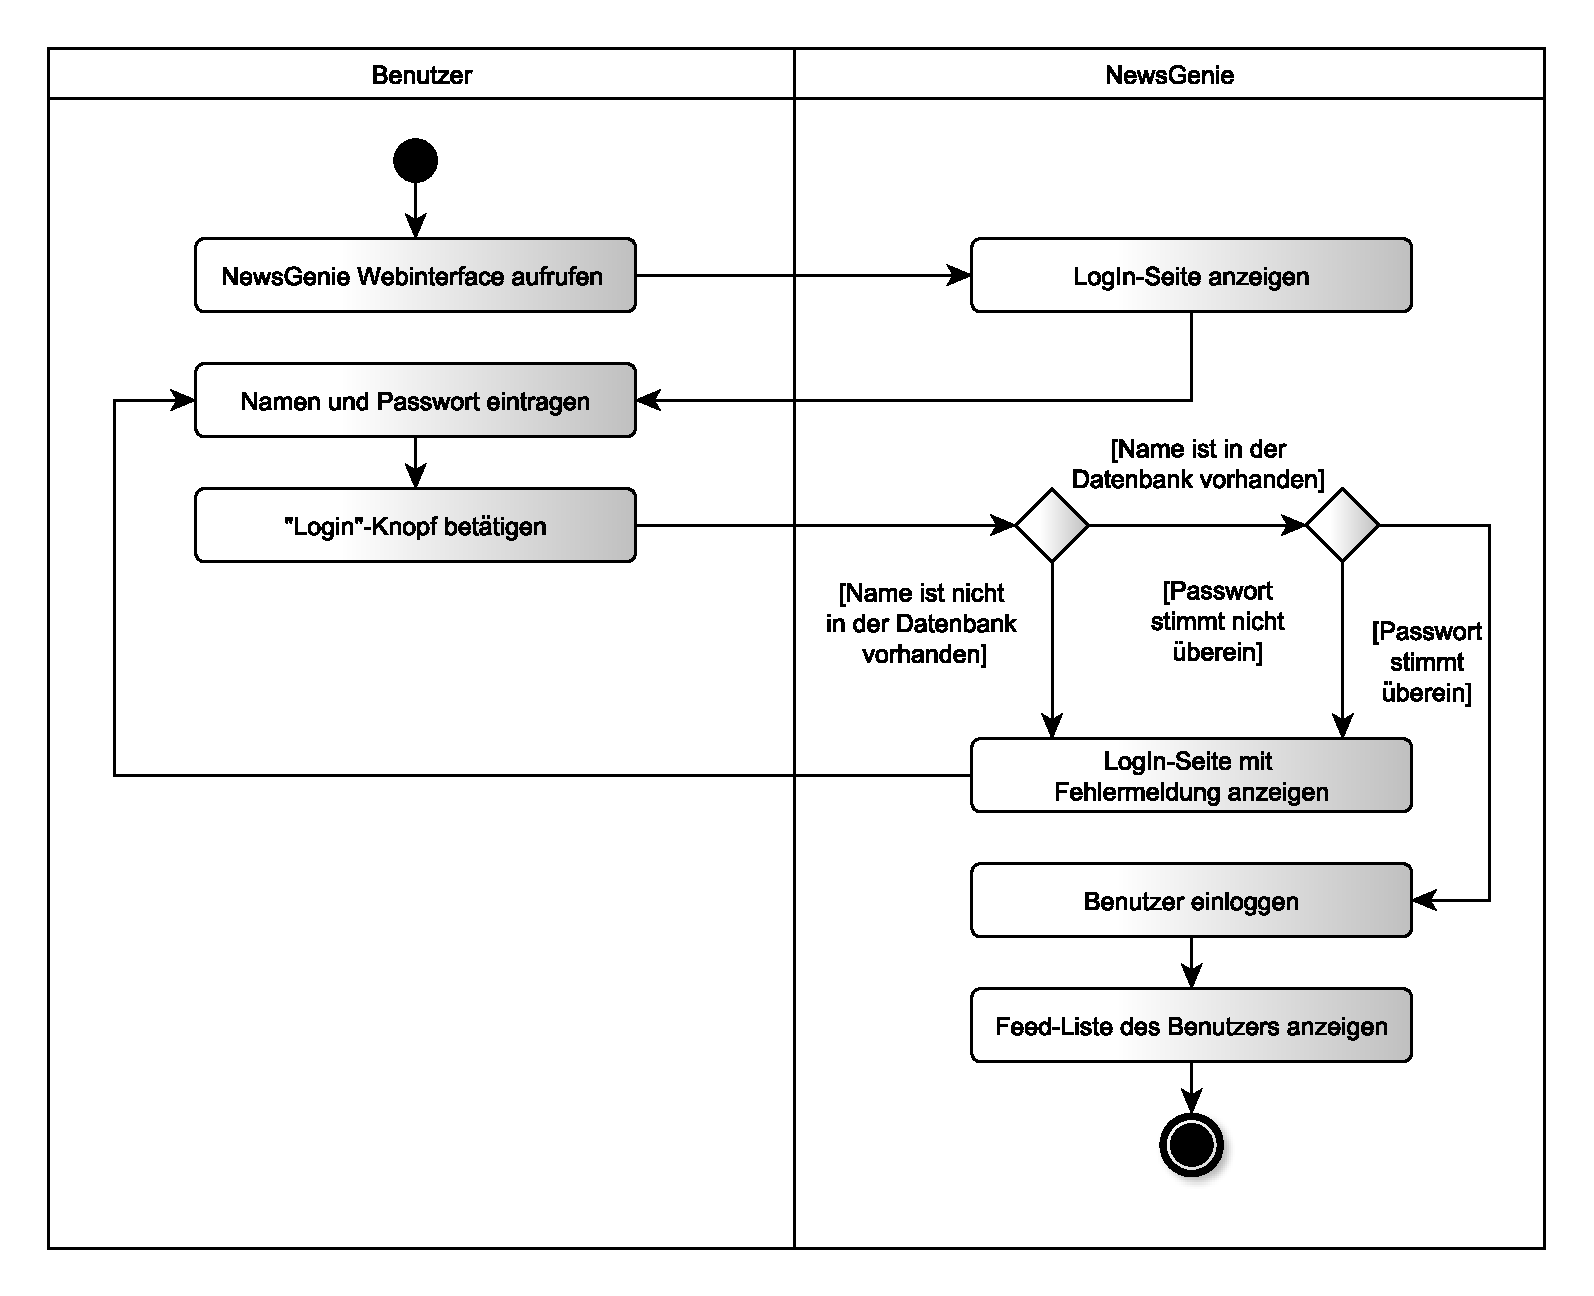
\includegraphics[width=1\textwidth]{Systementwurf/01_einleitung/weblogin.eps}
\caption{Aktivitätsdiagramm, \textit{Anmeldung am Webinterface}
\label{1.3}}
\end{figure}

\subsection{Feeds hinzufügen}

Sobald ein Benutzer sich am Webinterface eingeloggt hat, besteht für ihn die Möglichkeit, 
seine Feeds zu verwalten. Im nachfolgenden Aktivitätsdiagramm~\ref{1.4} wird dargestellt,
wie ein Benutzer neue Feeds abonnieren kann. Es reicht dazu aus, die URL des hinzuzufügenden 
Feeds in das dazu vorgesehene Textfeld einzugeben und die Eingabe per Knopfdruck zu bestätigen.
Das System prüft nun ob unter der angegebenen URL tatsächlich ein Feed zu finden ist und gibt sonst
eine Fehlermeldung aus. Falls der Feed existiert, wird er in der Datenbank gespeichert, falls dies noch nicht der Fall ist, und der Benutzer wird ihm als Abonnent zugeordnet.

\begin{figure}[h]
\centering
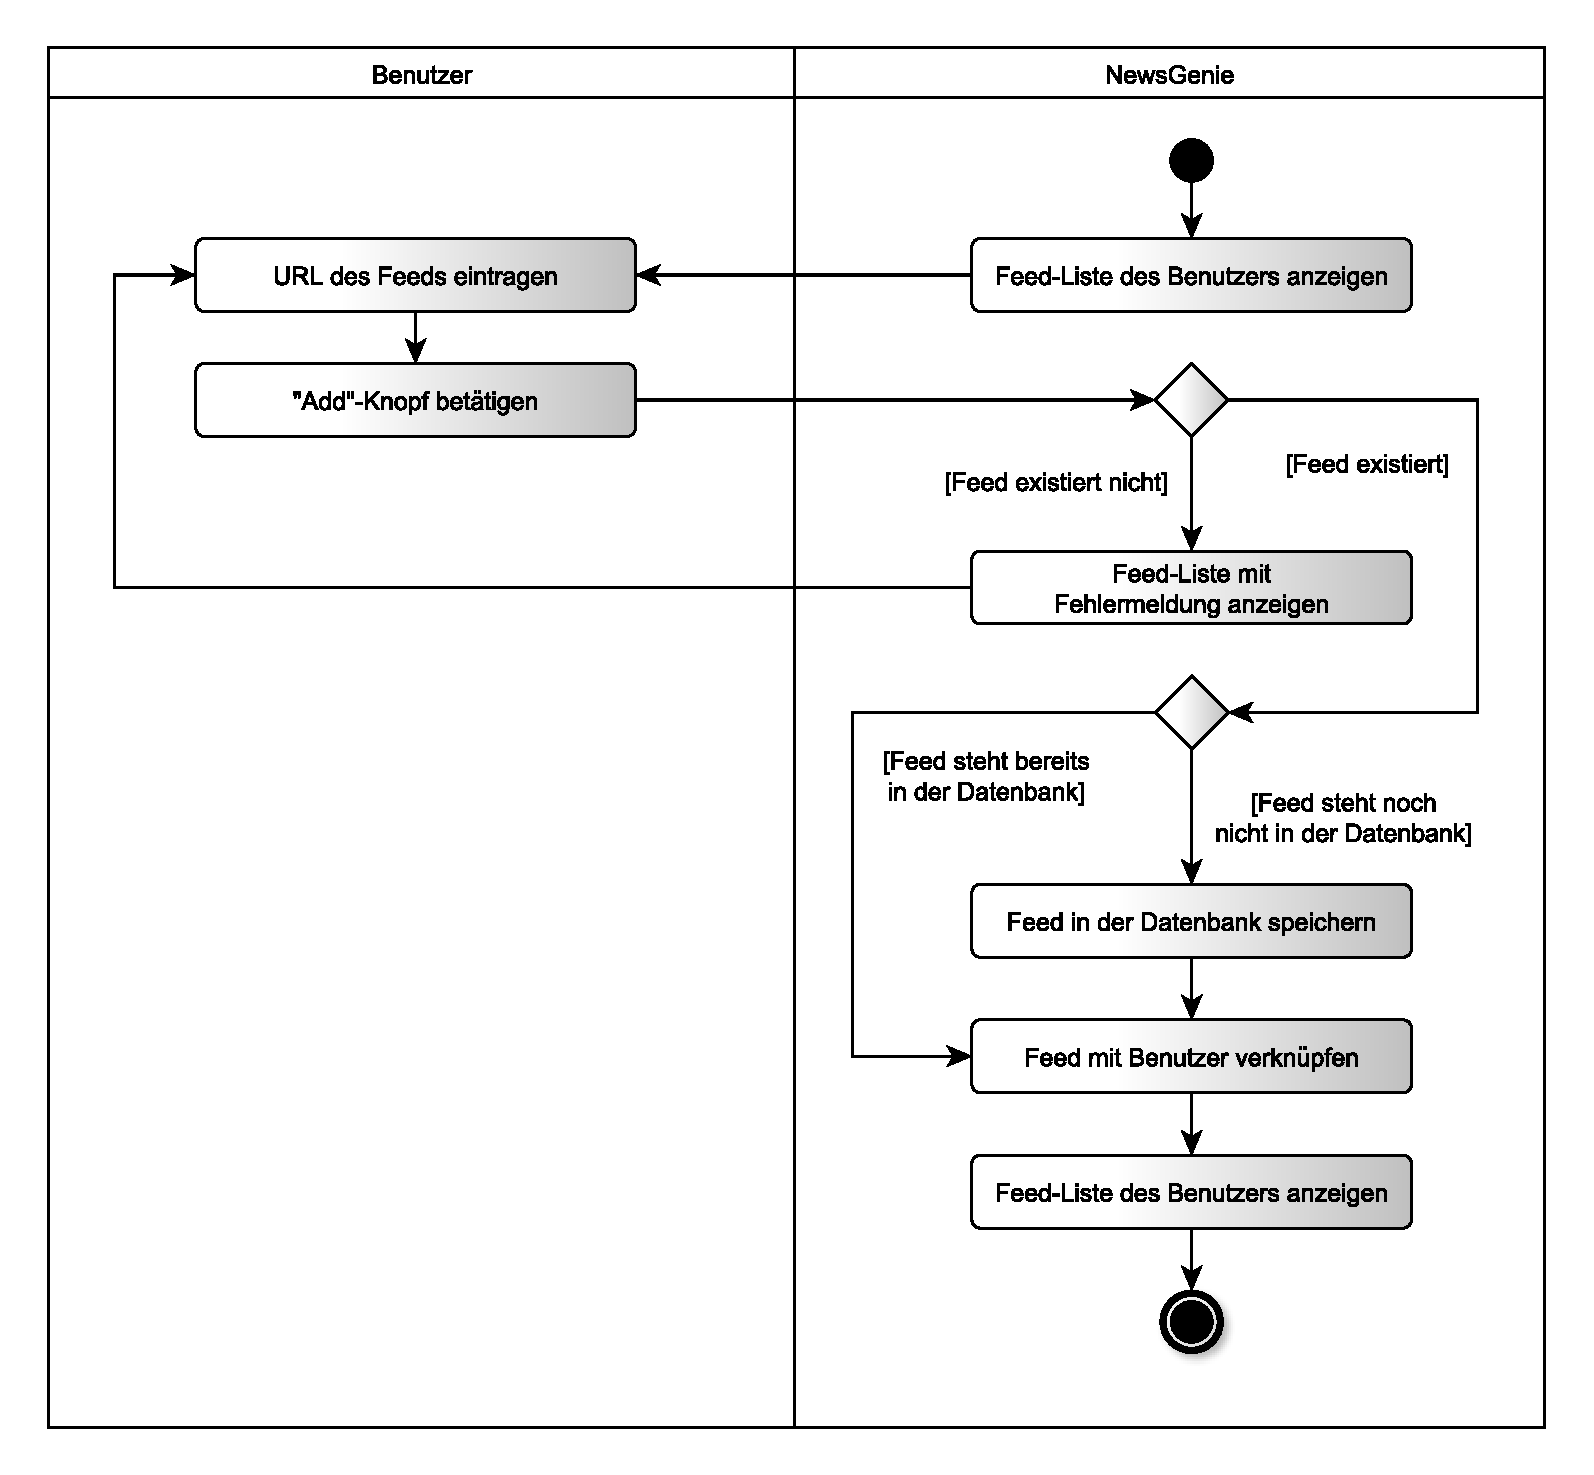
\includegraphics[width=1\textwidth]{Systementwurf/01_einleitung/addfeed.eps}
\caption{Aktivitätsdiagramm, \textit{Hinzufügen von Feeds}
\label{1.4}}
\end{figure}

\pagebreak[3]

\subsection{Interaktion zwischen Benutzer und Client}

Die verbale Kommunikation zwischen Benutzer und Client ist der Kern von \NewsGenie 
und zu komplex um sie komplett in einem Aktivitätsdiagramm darzustellen.
Folgende Funktionen sollen bereit gestellt werden:
\begin{itemize}
\item Login und Logout
\item Anfragen nach Neuigkeiten allgemein
\item Anfragen nach Neuigkeiten zu einem Thema
\item Erweiterung von Anfragen
\item Eingrenzung von Anfragen
\item Anfragen nach Fakten
\end{itemize}
Hierbei soll \NewsGenie möglichst selbstständig erkennen, was der Benutzer möchte und worauf sich
Anfragen beziehen. Insbesondere sol der Nutzer in der Lage sein, \NewsGenie zu jedem Zeitpunkt zu unterbrechen.

Ein relativ einfacher beispielhafter Workflow ist hierzu in Aktivitätsdiagramm~\ref{1.5} abgebildet.
Dieser Ablauf ist dabei nur einer von vielen. Durch die Kommunikation mittels Sprache hat der Nutzer zu jeder Zeit
viele verschiedene Möglichkeiten den Ablauf zu verändern.
Zusätzlich kann es immer passieren, dass Eingaben nicht verstanden werden und \NewsGenie nachfragen muss.
Die Verarbeitung einer Anfrage wird in Aktivitätsdiagramm~\ref{1.6} dargestellt.

\begin{figure}[h]
\centering
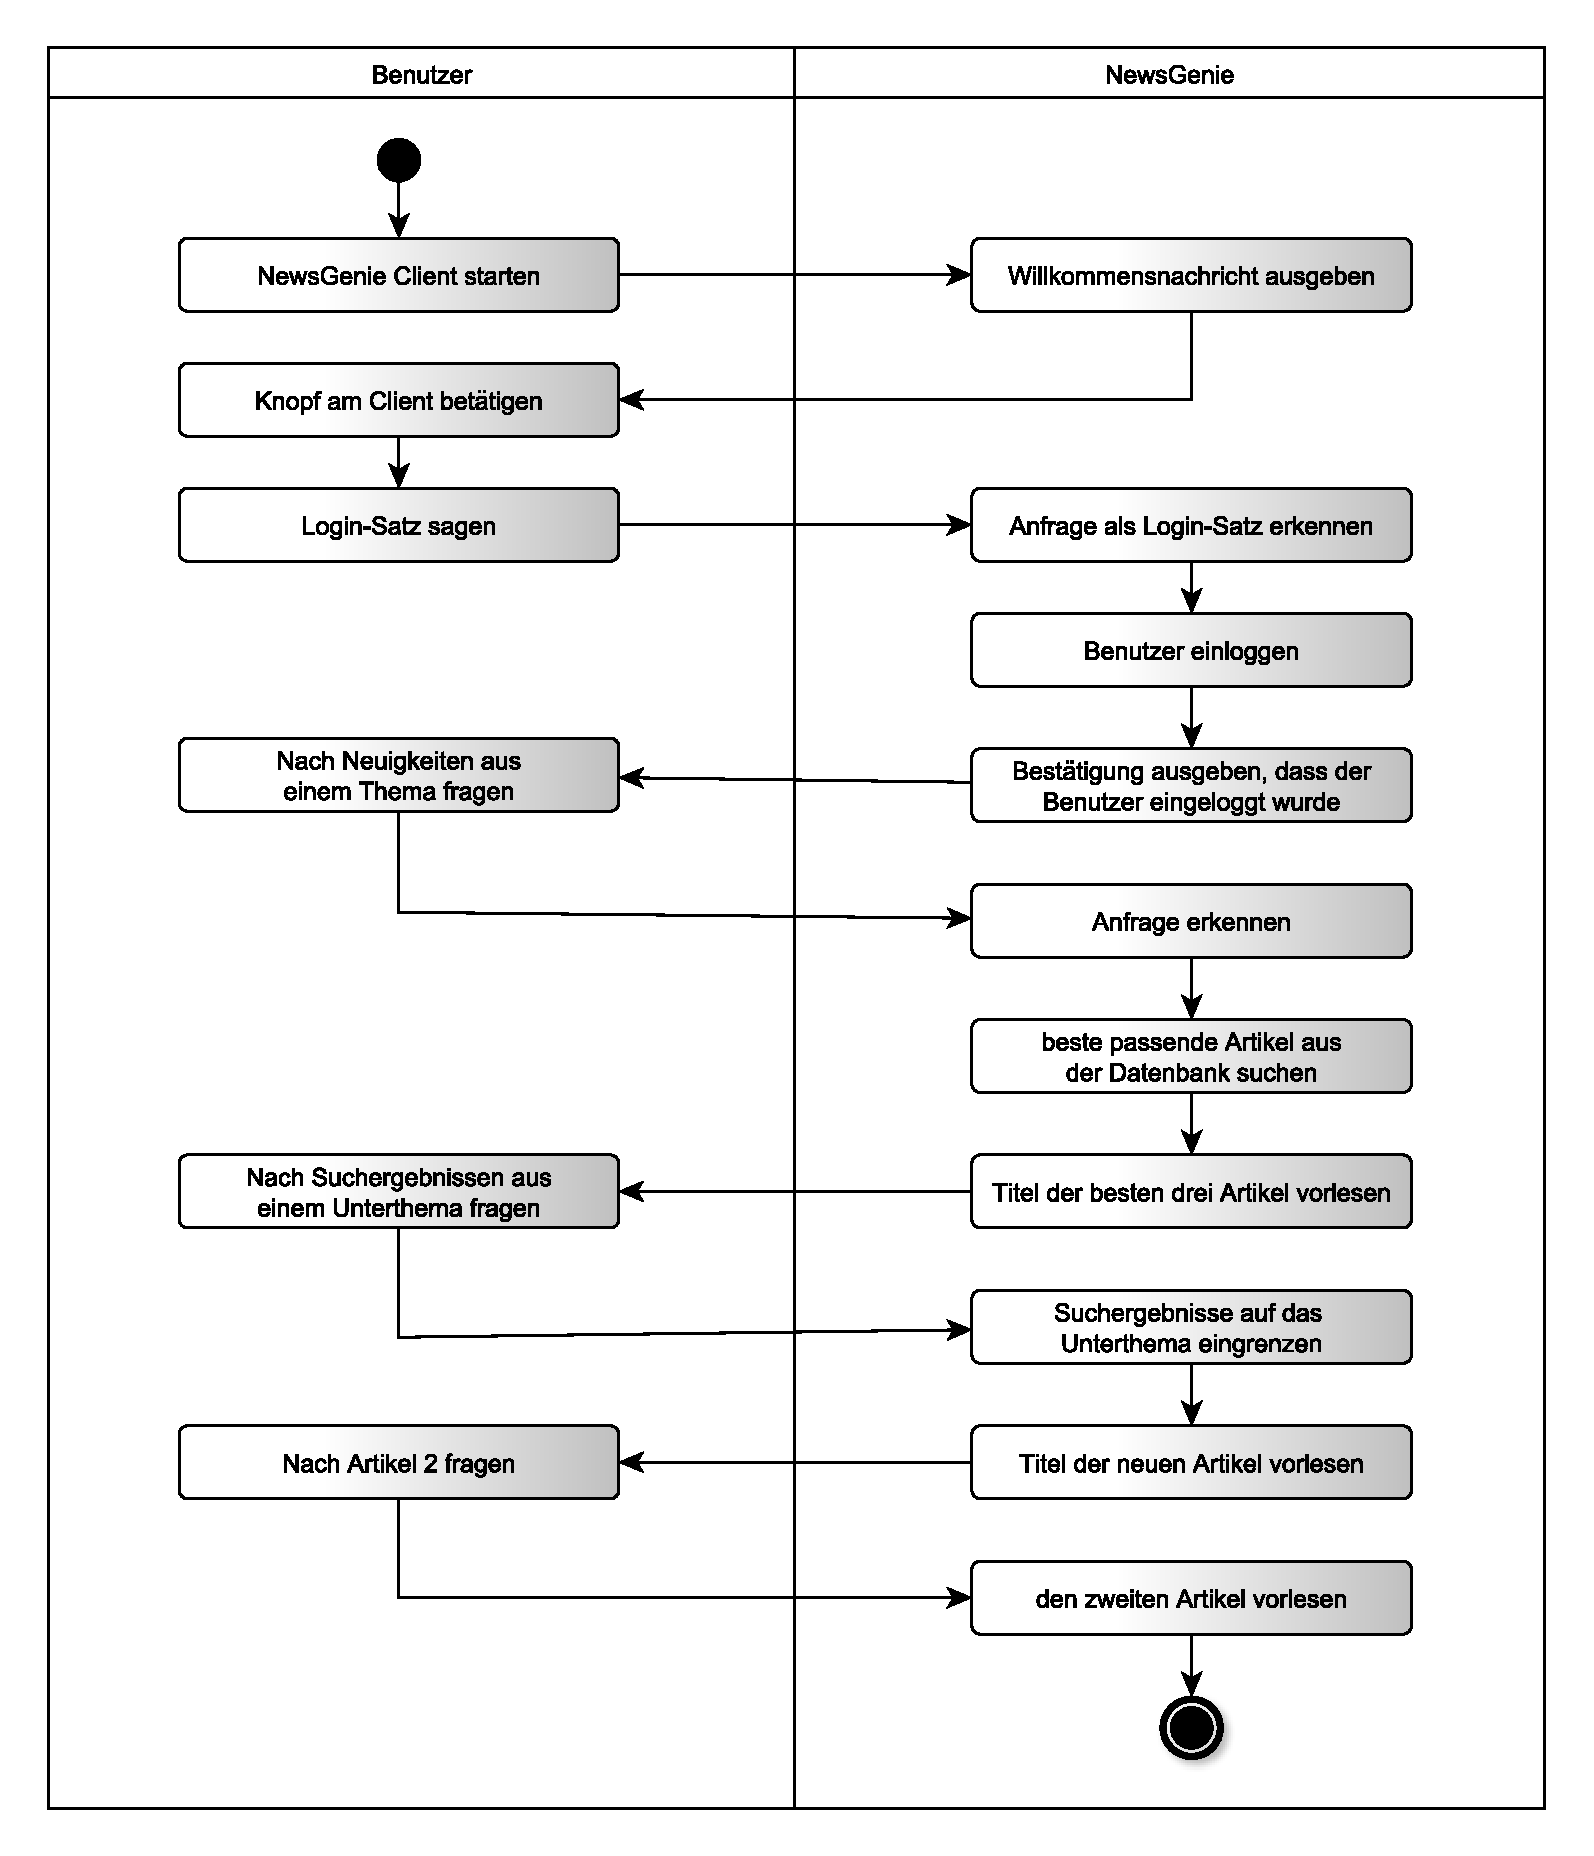
\includegraphics[width=1\textwidth]{Systementwurf/01_einleitung/conversation.eps}
\caption{Aktivitätsdiagramm, \textit{Beispielhafte Kommunikation mit dem Client}
\label{1.5}}
\end{figure}

\begin{figure}[h]
\centering
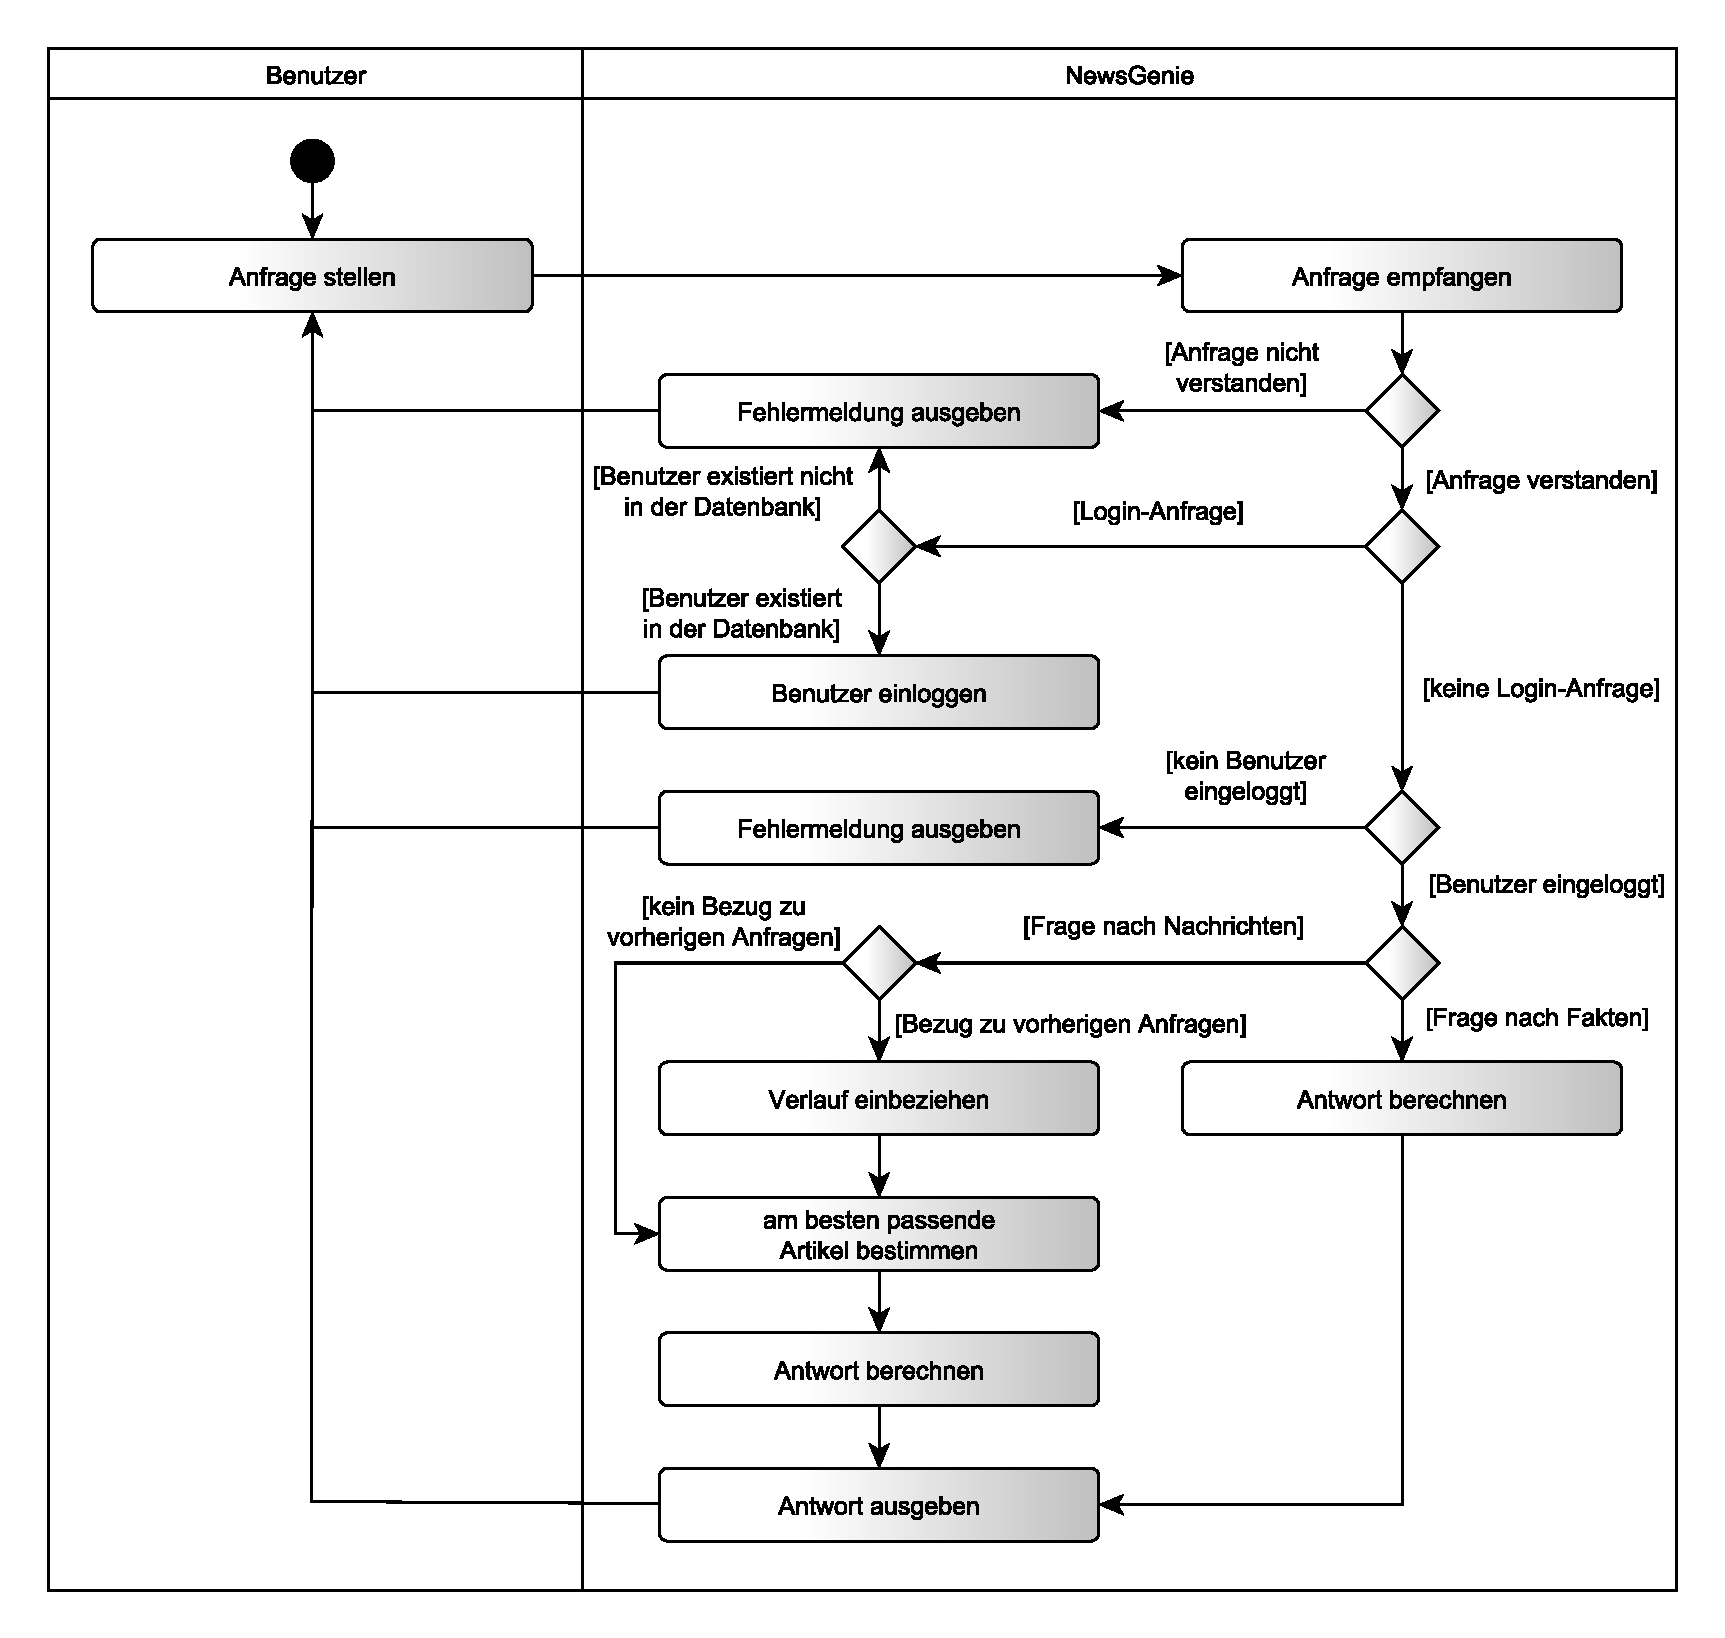
\includegraphics[width=1\textwidth]{Systementwurf/01_einleitung/request.eps}
\caption{Aktivitätsdiagramm, \textit{Verarbeitung einer Anfrage}
\label{1.6}}
\end{figure}

\iffalse
Die zwei Aktivitätsdiagramme in Abbildung \todo[inline]{Referenz} und
\todo[inline]{Referenz} zeigen den Workflow von \NewsGenies Hauptaufgabe, dem
Stellen einer Anfrage an das System.
Hierbei wird vorausgesetzt, dass sich der Nutzer bereits registriert und
entweder (je nach Anfragetyp) am Client oder im Webinterface angemeldet hat.
Will der Nutzer nun eine Anfrage am Client an \NewsGenie stellen, so spricht er
seine Frage. Die Anfrage durchläuft das System und eine Antwort wird
anschließend durch den Client ausgegeben. Dabei hängt die Antwort von dem
Ergebnis der Speech-To-Text- und der eigenen Analyse ab. Kann \NewsGenie zum
Beispiel keine Eingabe bzw. Frage feststellen, so gibt er eine entsprechende
Antwort mit Aufforderung zur Wiederholung der Eingabe auf.
Will der Nutzer stattdessen eine Anfrage im Webinterface an \NewsGenie stellen,
so tippt er seine Frage in das entsprechende Textfeld seine Frage. Nach dem
Klicken auf den "`Ask"'-Button, durchläuft die Anfrage genauso wie beim Client
das System und eine Antwort wird anschließend durch den Client ausgegeben.
Allerdings ist die Wahrscheinlichtkeit einer erfolgreichen Frage hier höher, da
Speech-To-Text hier nicht gebraucht und so die Fehlerwahrscheinlichkeit
minimiert wird.


\todo[inline]{Diagramm 1 - Client}
\todo[inline]{Diagramm 2 - Webinterface}
\fi